\documentclass[a4paper,12pt]{article} % добавить leqno в [] для нумерации слева
\usepackage[a4paper,top=1.3cm,bottom=2cm,left=1.5cm,right=1.5cm,marginparwidth=0.75cm]{geometry}
%%% Работа с русским языком
\usepackage{cmap}					% поиск в PDF
\usepackage{mathtext} 				% русские буквы в фомулах
\usepackage[T2A]{fontenc}			% кодировка
\usepackage[utf8]{inputenc}			% кодировка исходного текста
\usepackage[english,russian]{babel}	% локализация и переносы

\usepackage{graphicx}

\usepackage{wrapfig}
\usepackage{tabularx}

\usepackage{hyperref}
\usepackage[rgb]{xcolor}
\hypersetup{
colorlinks=true,urlcolor=blue
}
\usepackage{multirow}
\usepackage{hhline}


%%% Дополнительная работа с математикой
\usepackage{amsmath,amsfonts,amssymb,amsthm,mathtools} % AMS
\usepackage{icomma} % "Умная" запятая: $0,2$ --- число, $0, 2$ --- перечисление

%% Номера формул
\mathtoolsset{showonlyrefs=true} % Показывать номера только у тех формул, на которые есть \eqref{} в тексте.

%% Шрифты
\usepackage{euscript}	 % Шрифт Евклид
\usepackage{mathrsfs} % Красивый матшрифт

%% Свои команды
\DeclareMathOperator{\sgn}{\mathop{sgn}}

%% Перенос знаков в формулах (по Львовскому)
\newcommand*{\hm}[1]{#1\nobreak\discretionary{}
{\hbox{$\mathsurround=0pt #1$}}{}}

\begin{document}
	
	\begin{titlepage}
	\begin{center}
		{\large МОСКОВСКИЙ ФИЗИКО-ТЕХНИЧЕСКИЙ ИНСТИТУТ (НАЦИОНАЛЬНЫЙ ИССЛЕДОВАТЕЛЬСКИЙ УНИВЕРСИТЕТ)}
	\end{center}
	\begin{center}
		{\large Кафедра твердотельной электроники и радиофизики}
	\end{center}
	
	
	\vspace{4.5cm}
	{\huge
		\begin{center}
			{Лабораторная работа № 3}\\
			\textbf{определение ширины запрещенной зоны
полупроводников по спектральной зависимости
собственной фотопроводимости}
		\end{center}
	}
	\vspace{2cm}
	\begin{flushright}
		{\LARGE Салтыкова Дарья \\
			\vspace{0.5cm}
			Б04-105}
	\end{flushright}
	\vspace{8cm}
	\begin{center}
		Долгопрудный 2024
	\end{center}
\end{titlepage}








\noindent \textbf{ \Large Цель работы:} Определение ширины запрещённой зоны различных материалов по спектральной зависимости собственной фотопроводимости;


\section{Теоретические сведения}
При воздействии на полупроводник излучения с энергией кванта $h\nu$, превышающей ширину запрещённой зоны $E_g$ в зоне проводимости, и соотвественно в валентной зоне возникают неравновесные электроны и дырки. Их появление связано с переходами электронов из валентной зоны проводимости. В результате увеличивается проводимость кристалла. Это явление называется собственной фотопроводимостью.

В непрямозонных полупроводниках типа германия и кремния минимум зоны проводимости и максимум валентной зоны расположены в различных точках зоны Бриллюэна. В этом случае оптический переход электрона из вершины валентной зоны в минимум зоны проводимости возможен лишь при участии третьей частицы – фонона. В соответствии с законом сохранения импульса квазиимпульс такого фонона $q_{\text{ф}}\approx\hbar k_{\text{Б}}$, а энергия $\hbar\omega$ должна удовлетворять закону сохранения энергии:
\begin{equation}
    h\nu = E_g\pm \hbar\omega_q+\hbar^2(k_n-k_c)^2/2m_n+\hbar^2k_p^2/2m_p
\end{equation}
где $k_n$ и $k_p$ -- начальные волновые числа электрона и дырки, а $k_c$ -- конечное волновое число электрона.

Таким образом, край основной полосы поглощения в полупроводниках типа кремния и германия определяется непрямыми оптическими переходами, сопровождающимися поглощением и испусканием фононов. При этом для разрешённых переходов, которые доминируют в полупроводниках такого типа, коэффициент поглощения:

\begin{equation}
    K=C\left[\frac{(h\nu-E_g+\hbar\omega_q)^2}{\exp{\frac{\hbar\omega_q}{kT}}-1}+\frac{(h\nu-E_g-\hbar\omega_q)^2}{1-\exp{-\frac{\hbar\omega_q}{kT}}}\right]
\end{equation}
При больших энергиях квантов $h\nu>(E_g+\hbar\omega_q)$ начинают преобладать переходы с эмиссией фононов и зависимость $K^{1/2}$ от $h\nu$ должна аппроксимироваться прямой, пересекающей ось энергии в точке $h\nu_1=E_g+\hbar\omega_q$.

При рассмотрении случая сильного поглощения излечения в образце (оптически толстый образец), то есть при $d/K<<1$, где $d$ -- толщина образца, скорость генерации электронно-дырочных пар экспоненциально уменьшается от поверхности вглубь образца:
\begin{equation}
    g(x)\approx K(1-R)N_0\exp{-Kx}
\end{equation}
где $R$ -- коэффициент отражения света, а $N_0$ -- поток квантов на единицу поверхности.

Неоднородная германия электронов и дырок в направлении освещения приводит к появлению диффузионно-дрейфовых потоков носителей заряда: быстро диффундирующие носители (электроны) опережают медленные (дырки), что приводит к возникновению электрического поля, ускоряющего медленные носители и замедляющего быстрые и к появлению дрейфовых составляющих потоков. При этом изменение проводимости $\Delta\Sigma$ существенным образом зависит от граничных условий на поверхности образца:
\begin{equation}
    \Delta\Sigma\sim N_0\left(1+\frac{S}{D}\frac{1}{K}\right)
\end{equation}
где $S$ -- скорость поверхностной рекомбинации, $D$ -- коэффициент амбиполярной диффузии.



\section{Экспериментальная установка}

Для изменения фотоответа полупроводника $\Delta\Sigma$ образец включается последовательно с нагрузочным сопротивлением и источником постоянного напряжения. При освещении проводимость образца возрастает, происходит перераспределение напряжение между образцом и нагрузкой. В результате падение напряжения $U$ на образце при малом относительном увеличении проводимости уменьшается на величину
    \begin{equation}
        \Delta U=\varepsilon\frac{R_H\cdot R_0^2}{(R_H+R_0)^2}\Delta\Sigma
        \label{eq:deltaU}
    \end{equation}
    где $\varepsilon$ -- постоянное напряжение, $R_H$ и $R_0$ -- сопротивление нагрузки и образца, $\Sigma$ -- проводимость.

    Для повышения чувствительности измерения обычно проводят при периодическом прерывании светового потока. При этом соотношение (\ref{eq:deltaU}) характеризует амплитуду отрицательных импульсов напряжения на концах образца. Для исследования интересующих нас зависимостей $\Delta\Sigma/N_0$ от энергии кванта $h\nu$ наряду с $\Delta U$ необходимо знать спектральное распределение интенсивности источника излучения $N_0(h\nu)$.
    \begin{figure}[!htb]
        \centering
        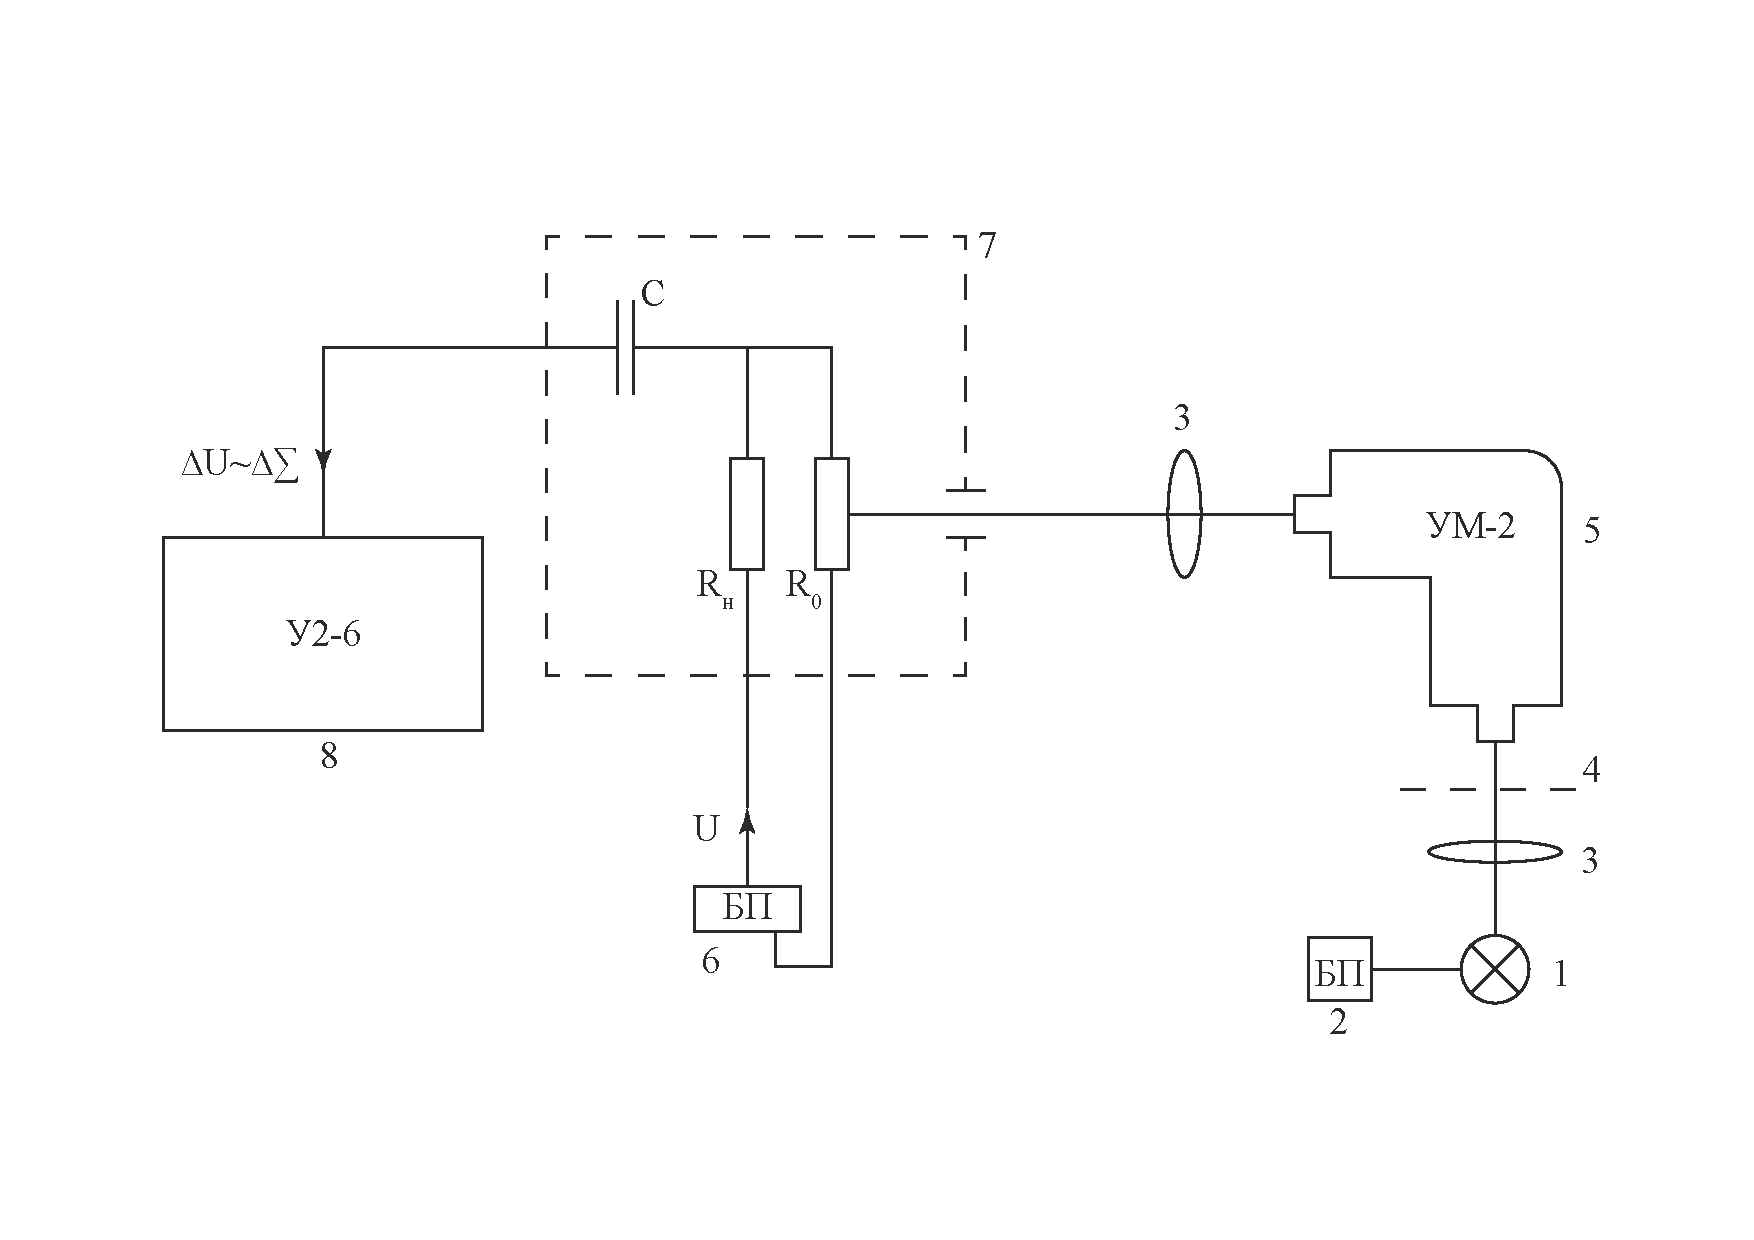
\includegraphics[width=\textwidth]{exp_scheme.pdf}
        \caption{Схема экспериментальной установки. 1 -- осветитель, 2 -- блок питания осветителя, 3 -- линзы, 4 -- механический модулятор излучения, 5 -- монохроматор, 6 -- блок питания образца, 7 -- схема включения образца, 8 -- усилитель}
    \end{figure}

\newpage

\section{Результаты измерений}




\subsection{Кремний}
Кремний - непрямозонный полупроводник. Построим зависимость корня фотоответа от энергии 
квантов. Наблюдаем два линейных участка (в области больших и малых энергий).
Найдем точки пересечения прямых с осью $x$ и взяв их средее значение получим ширину запрещенной зоны.


\begin{figure}[h!]
    \centering
    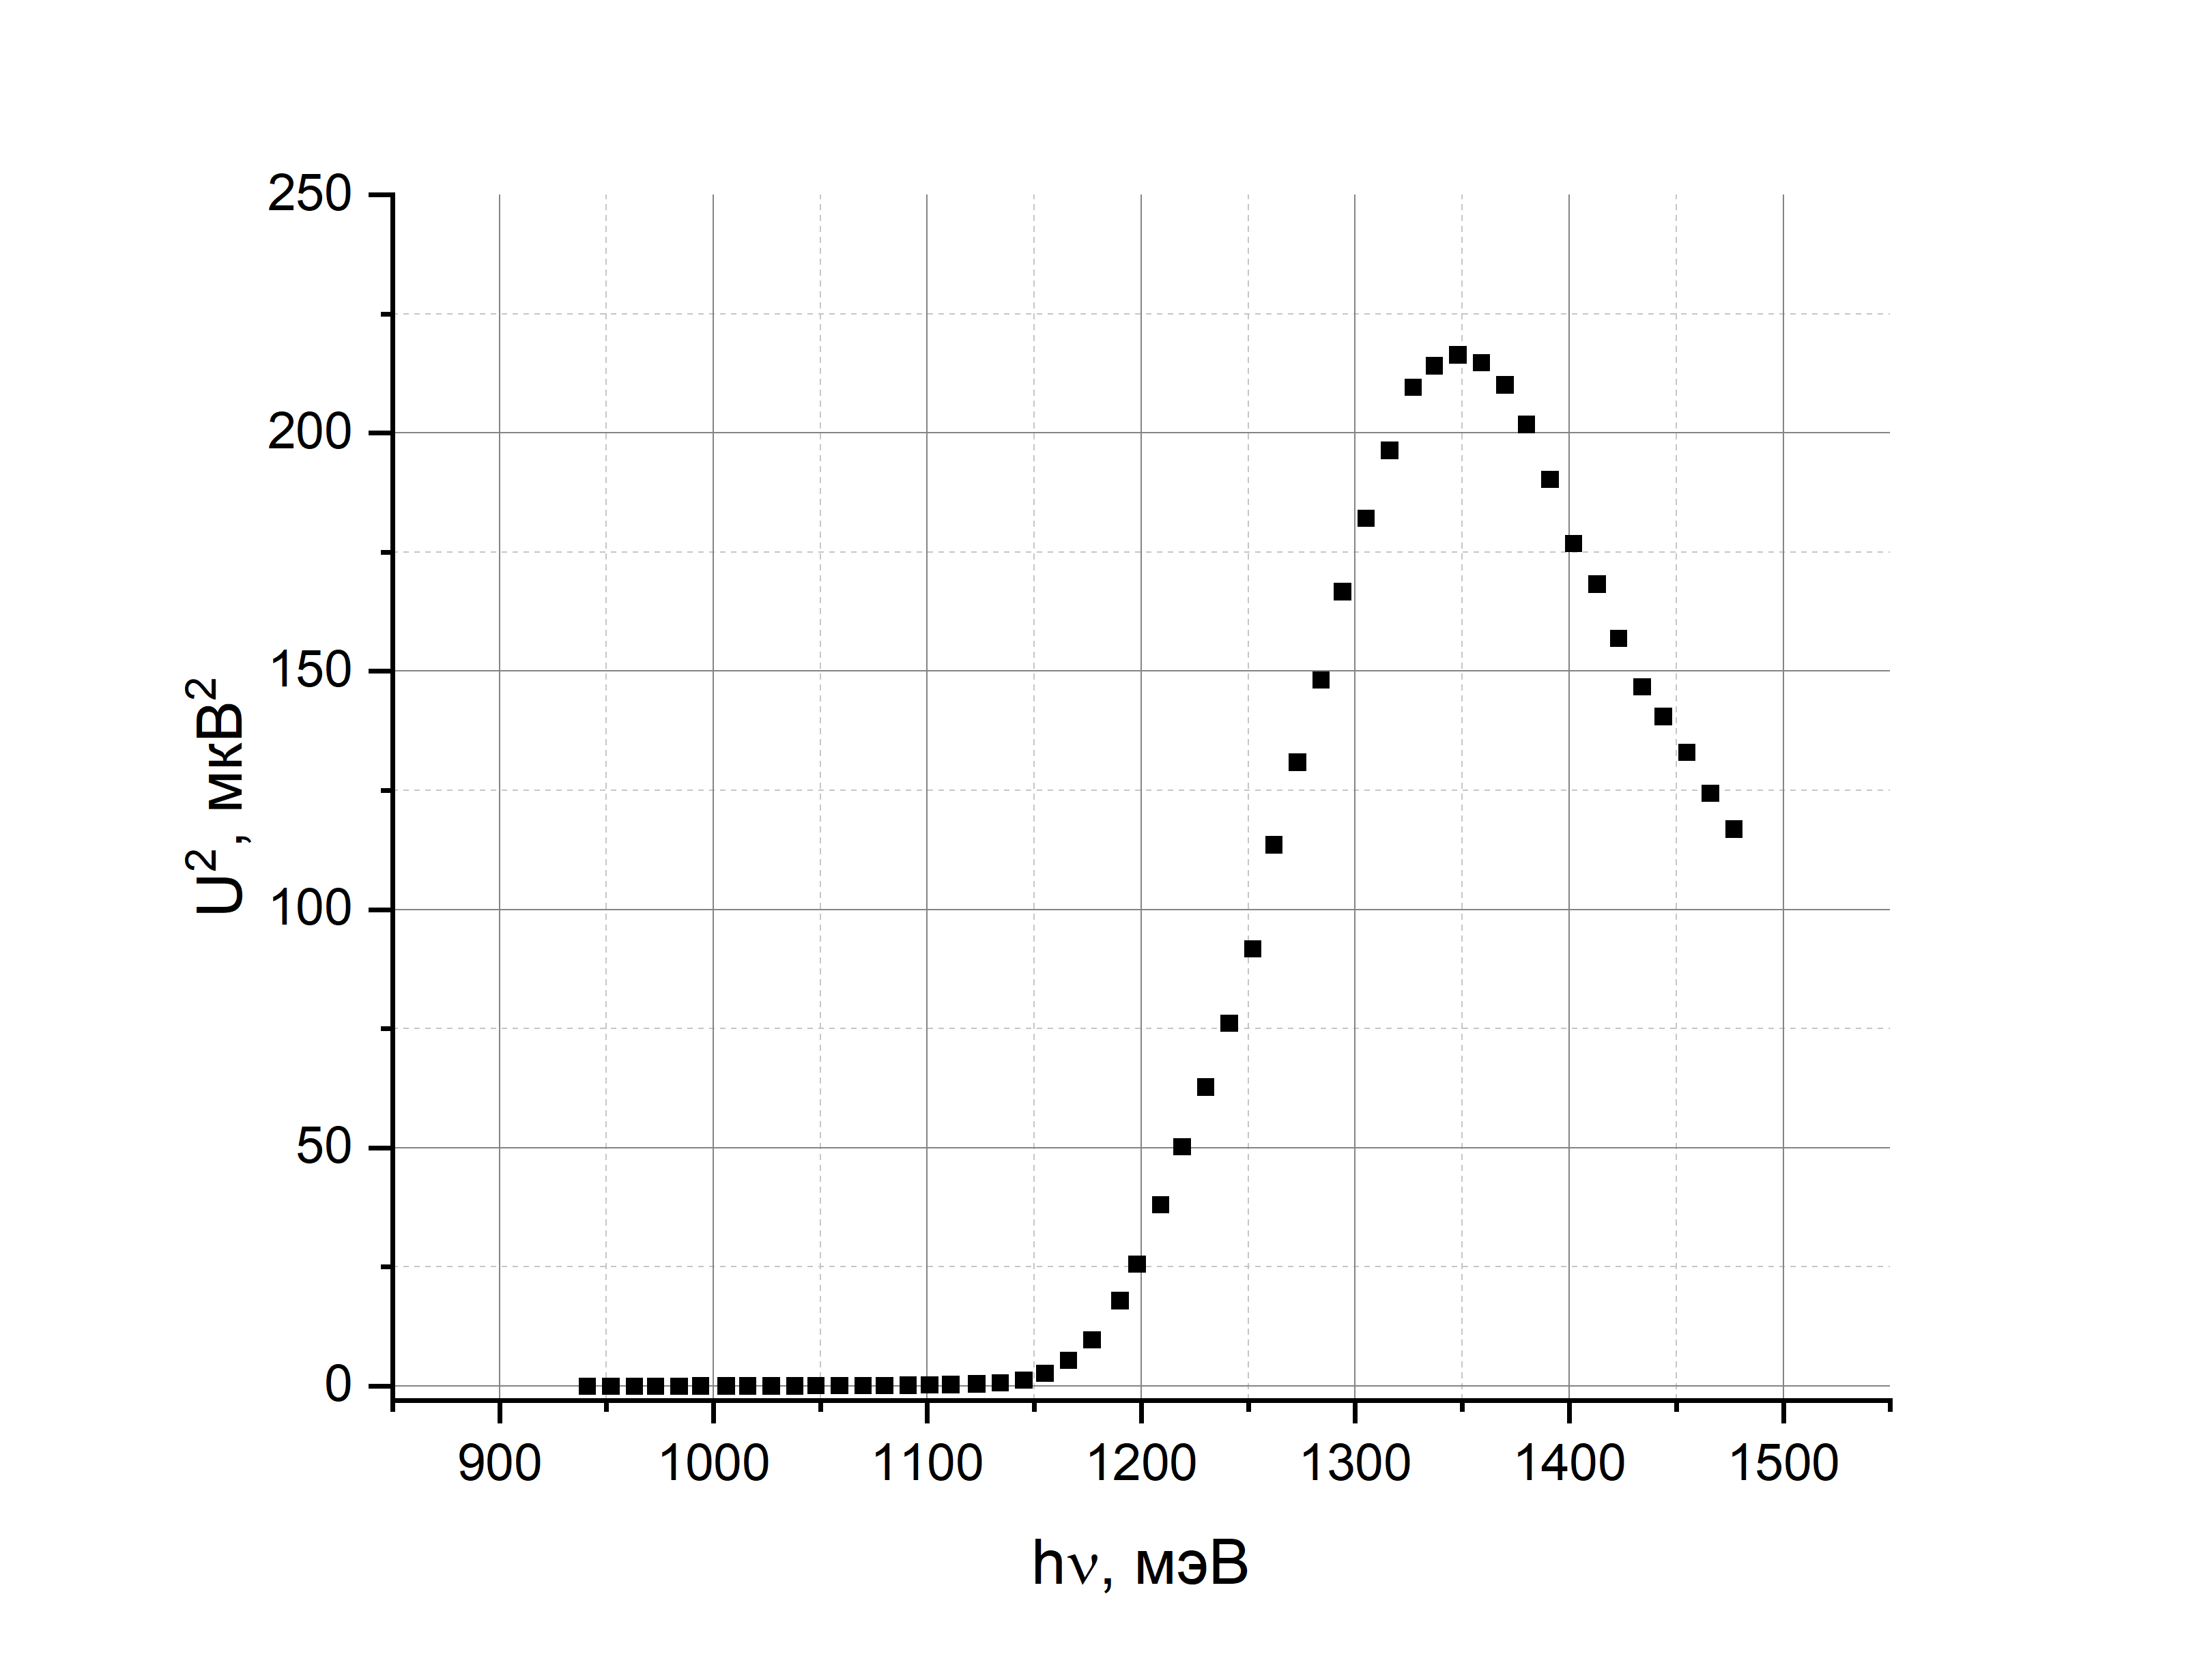
\includegraphics[width=0.69\textwidth]{Si_raw.png}
    \caption{Зависимость сигнала фотоответа Si от энергии падающего фотона}
    \label{fig:Si}
\end{figure}

\begin{figure}[h!]
    \centering
    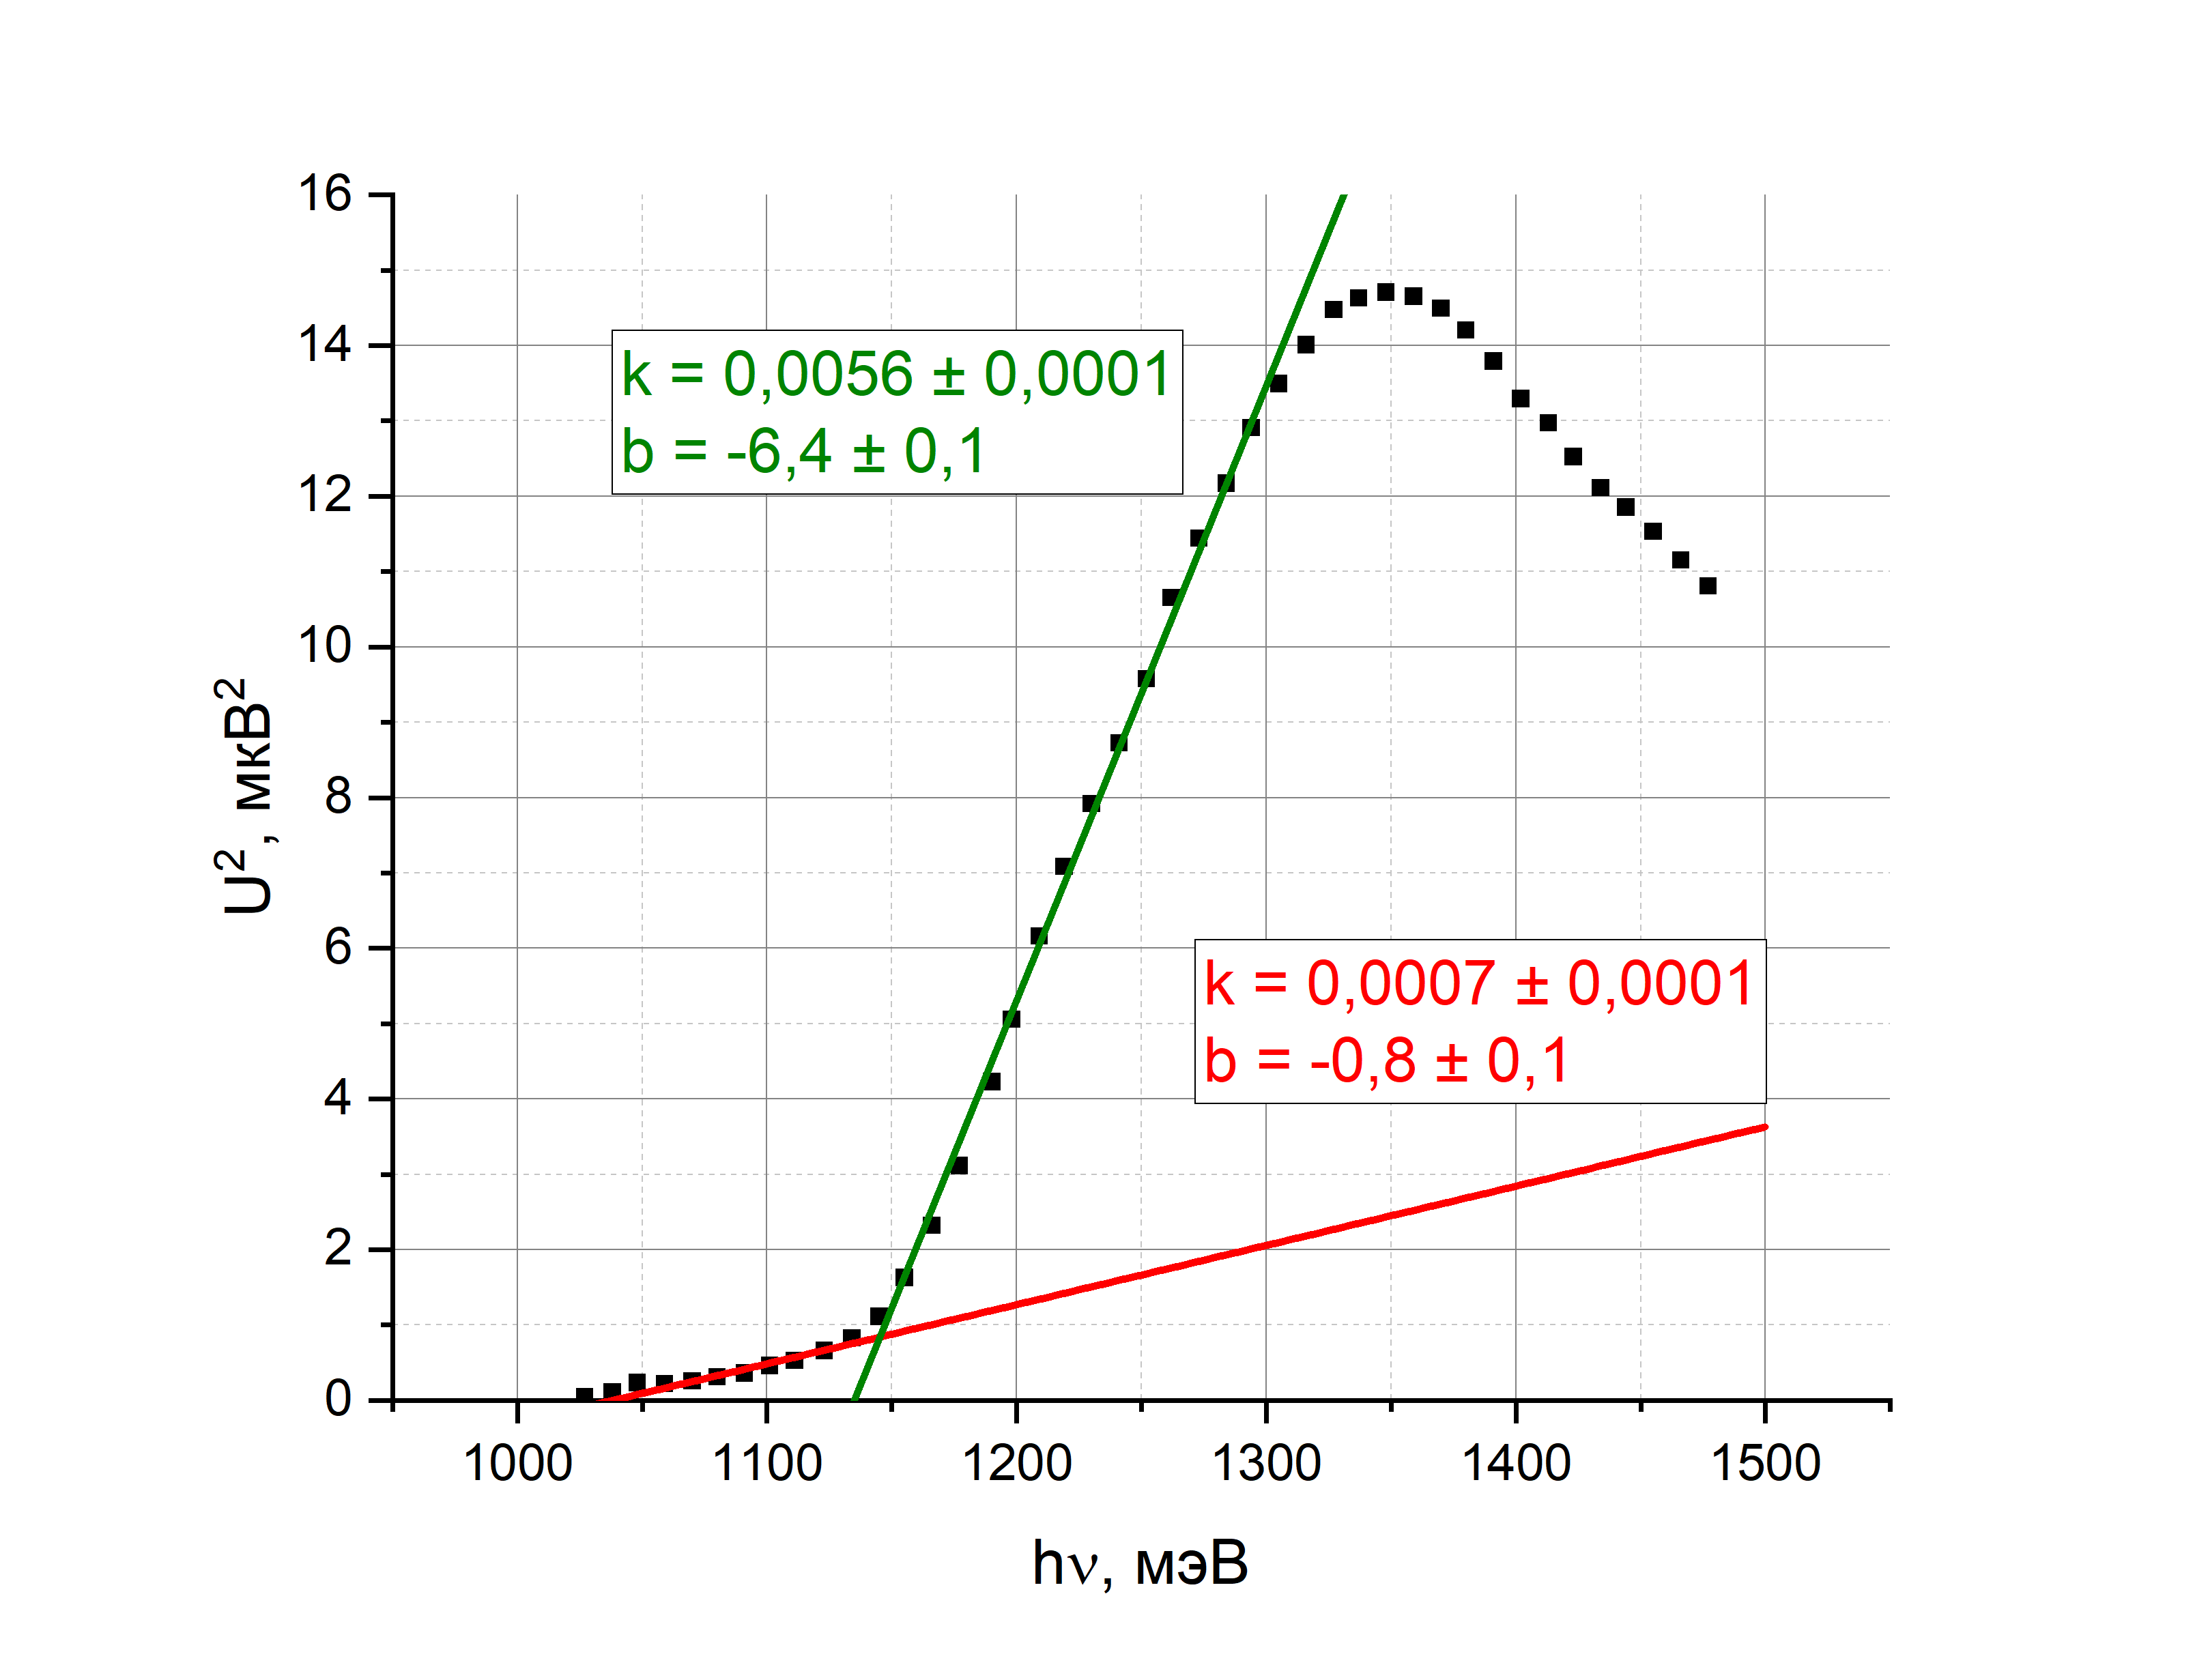
\includegraphics[width=0.69\textwidth]{Si.png}
    \caption{Определение ширины запрещенной зоны кремния}
    \label{fig:Si}
\end{figure}



Точки пересечения прямых с осью $x$ оказались равными: $x_{1} =  (1136 \pm 57) \text{ мэВ}, x_{2} = (1050 \pm 50) \text{ мэВ} $. Таким образом, ширина запрещенной зоны кремния: $ E_{g}^{Si} = (1100 \pm 50) \text{ мэВ}$.



\subsection{CdSe}
CdSe - прямозонный полупроводник. Для нахождения 
ширины запрещенной зоны построим зависимость квадрата фотоответа от энергии квантов.

\begin{figure}[h!]
    \centering
    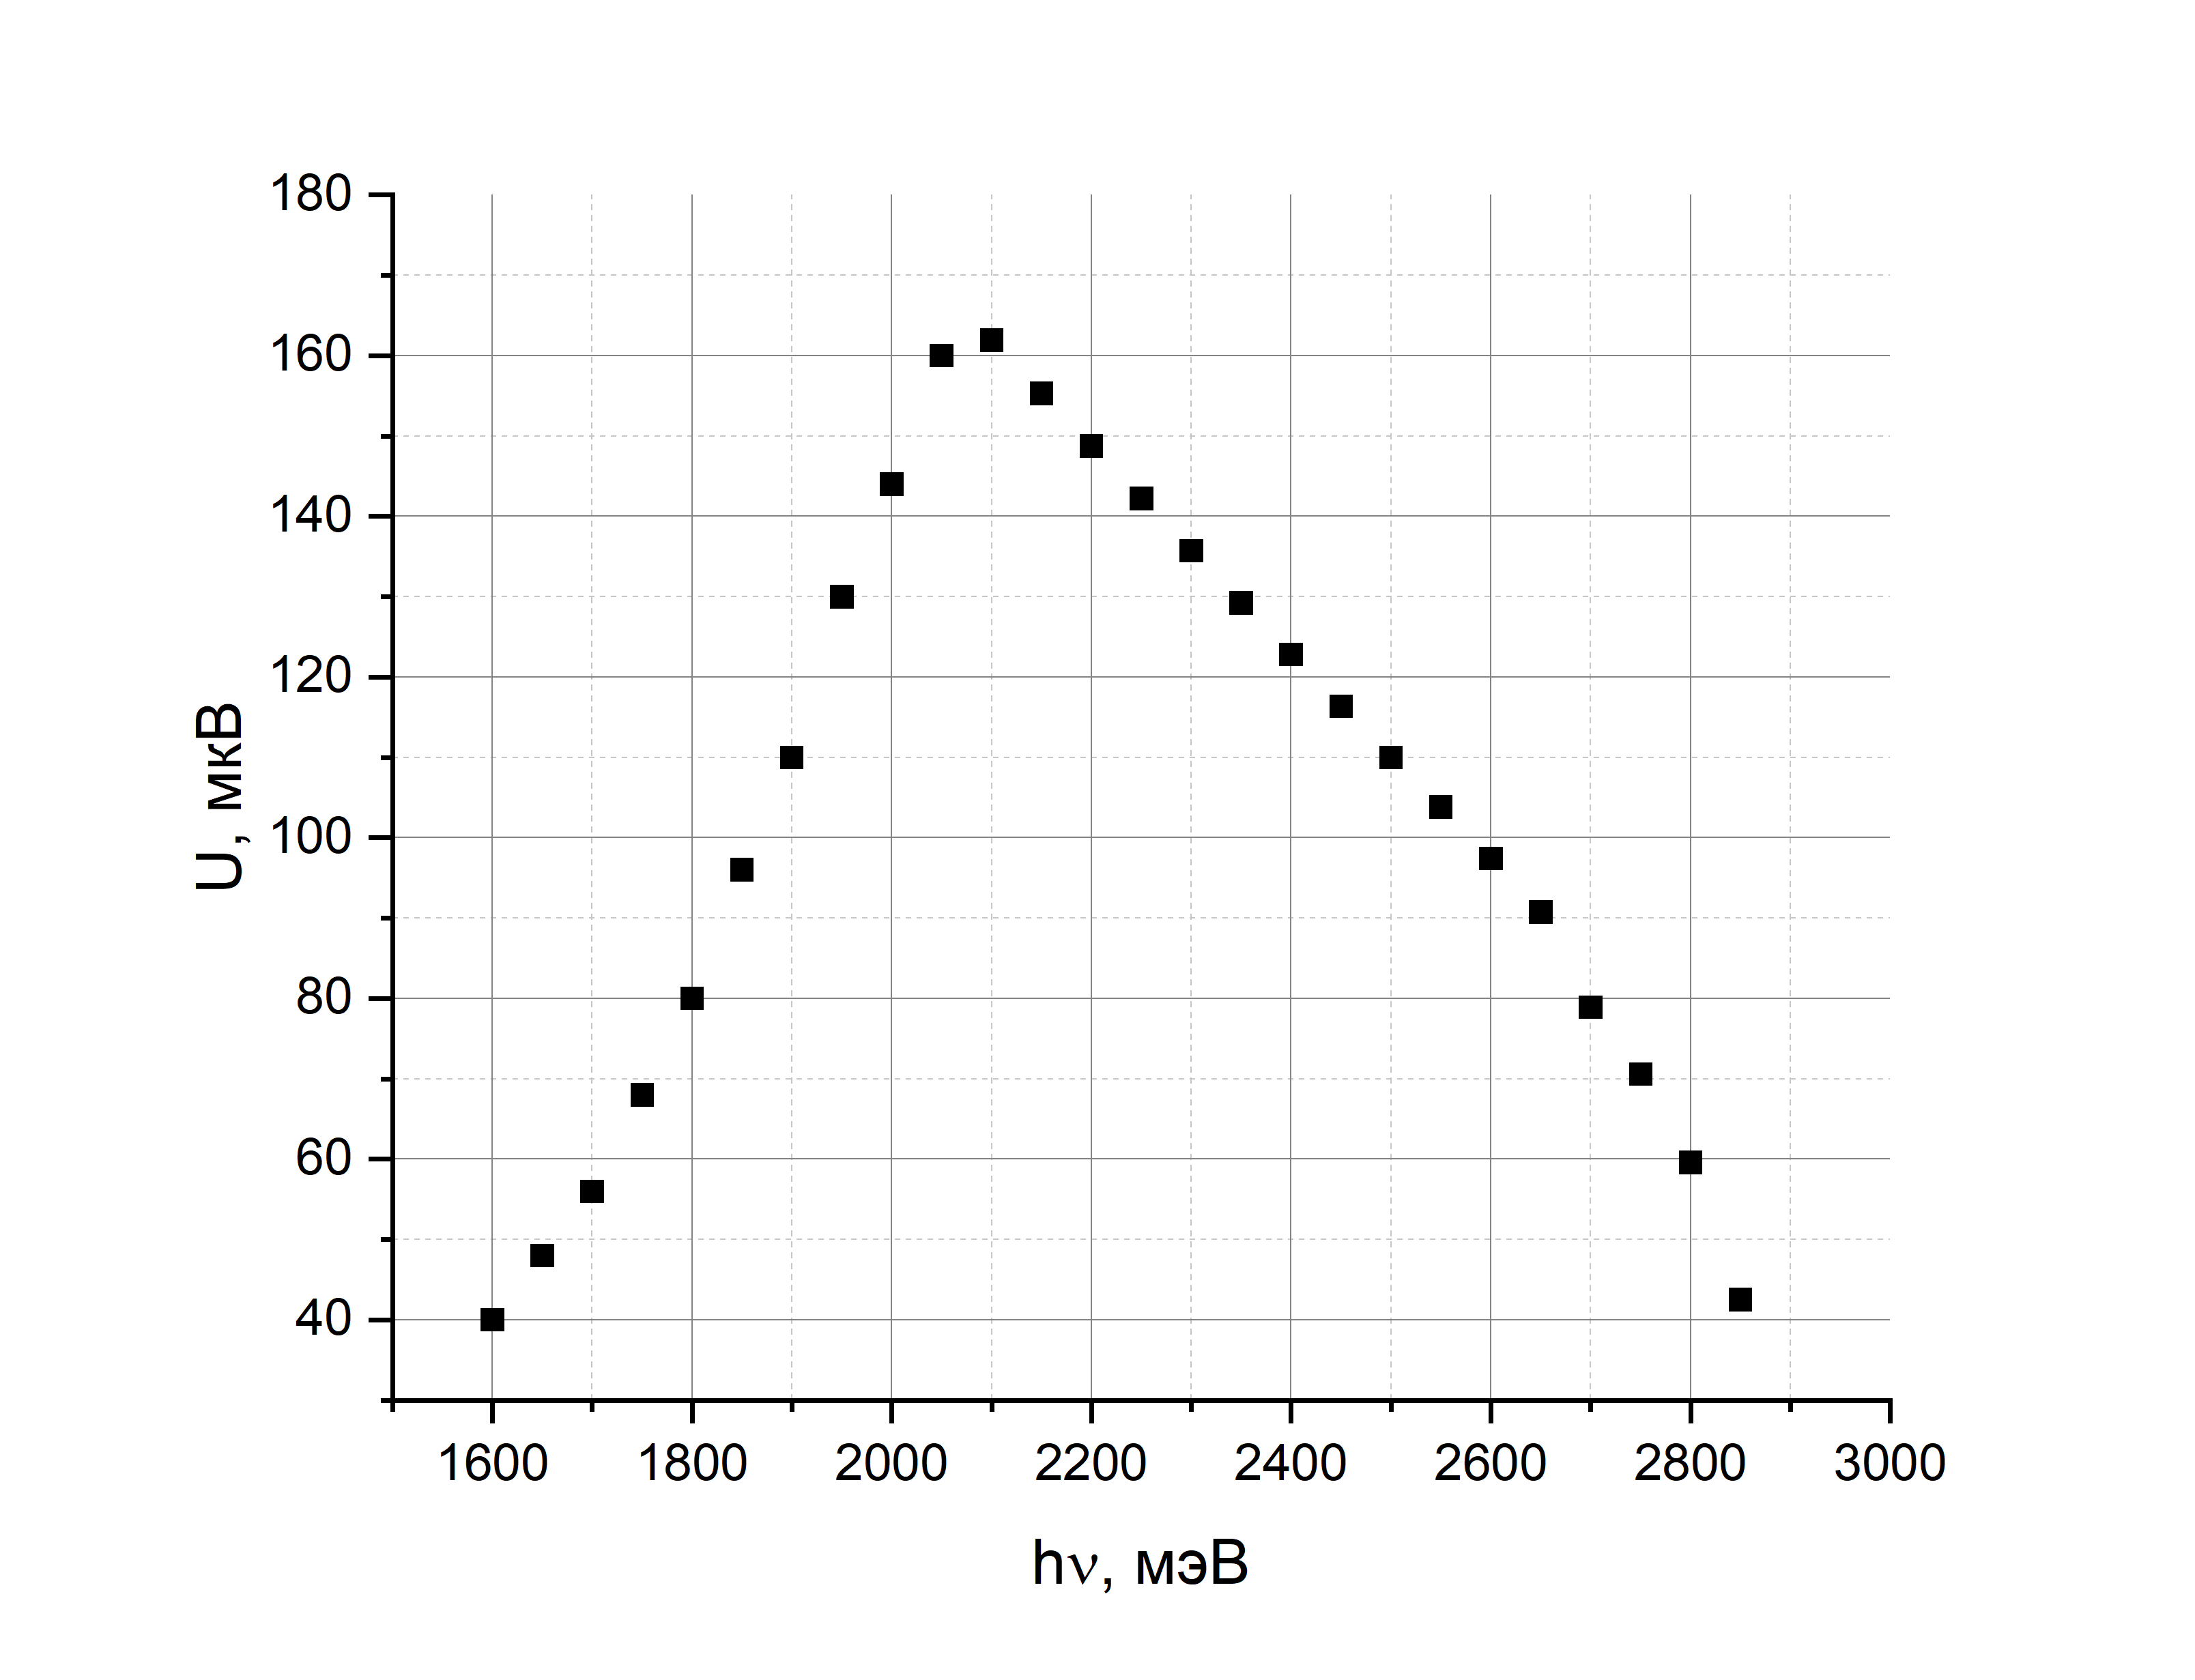
\includegraphics[width = 0.69\textwidth]{CdSe_raw.png}
    \caption{Зависимость сигнала фотоответа CdSe от энергии падающего фотона}
    \label{fig:CdSe_raw_data}
\end{figure}

\begin{figure}[h!]
    \centering
    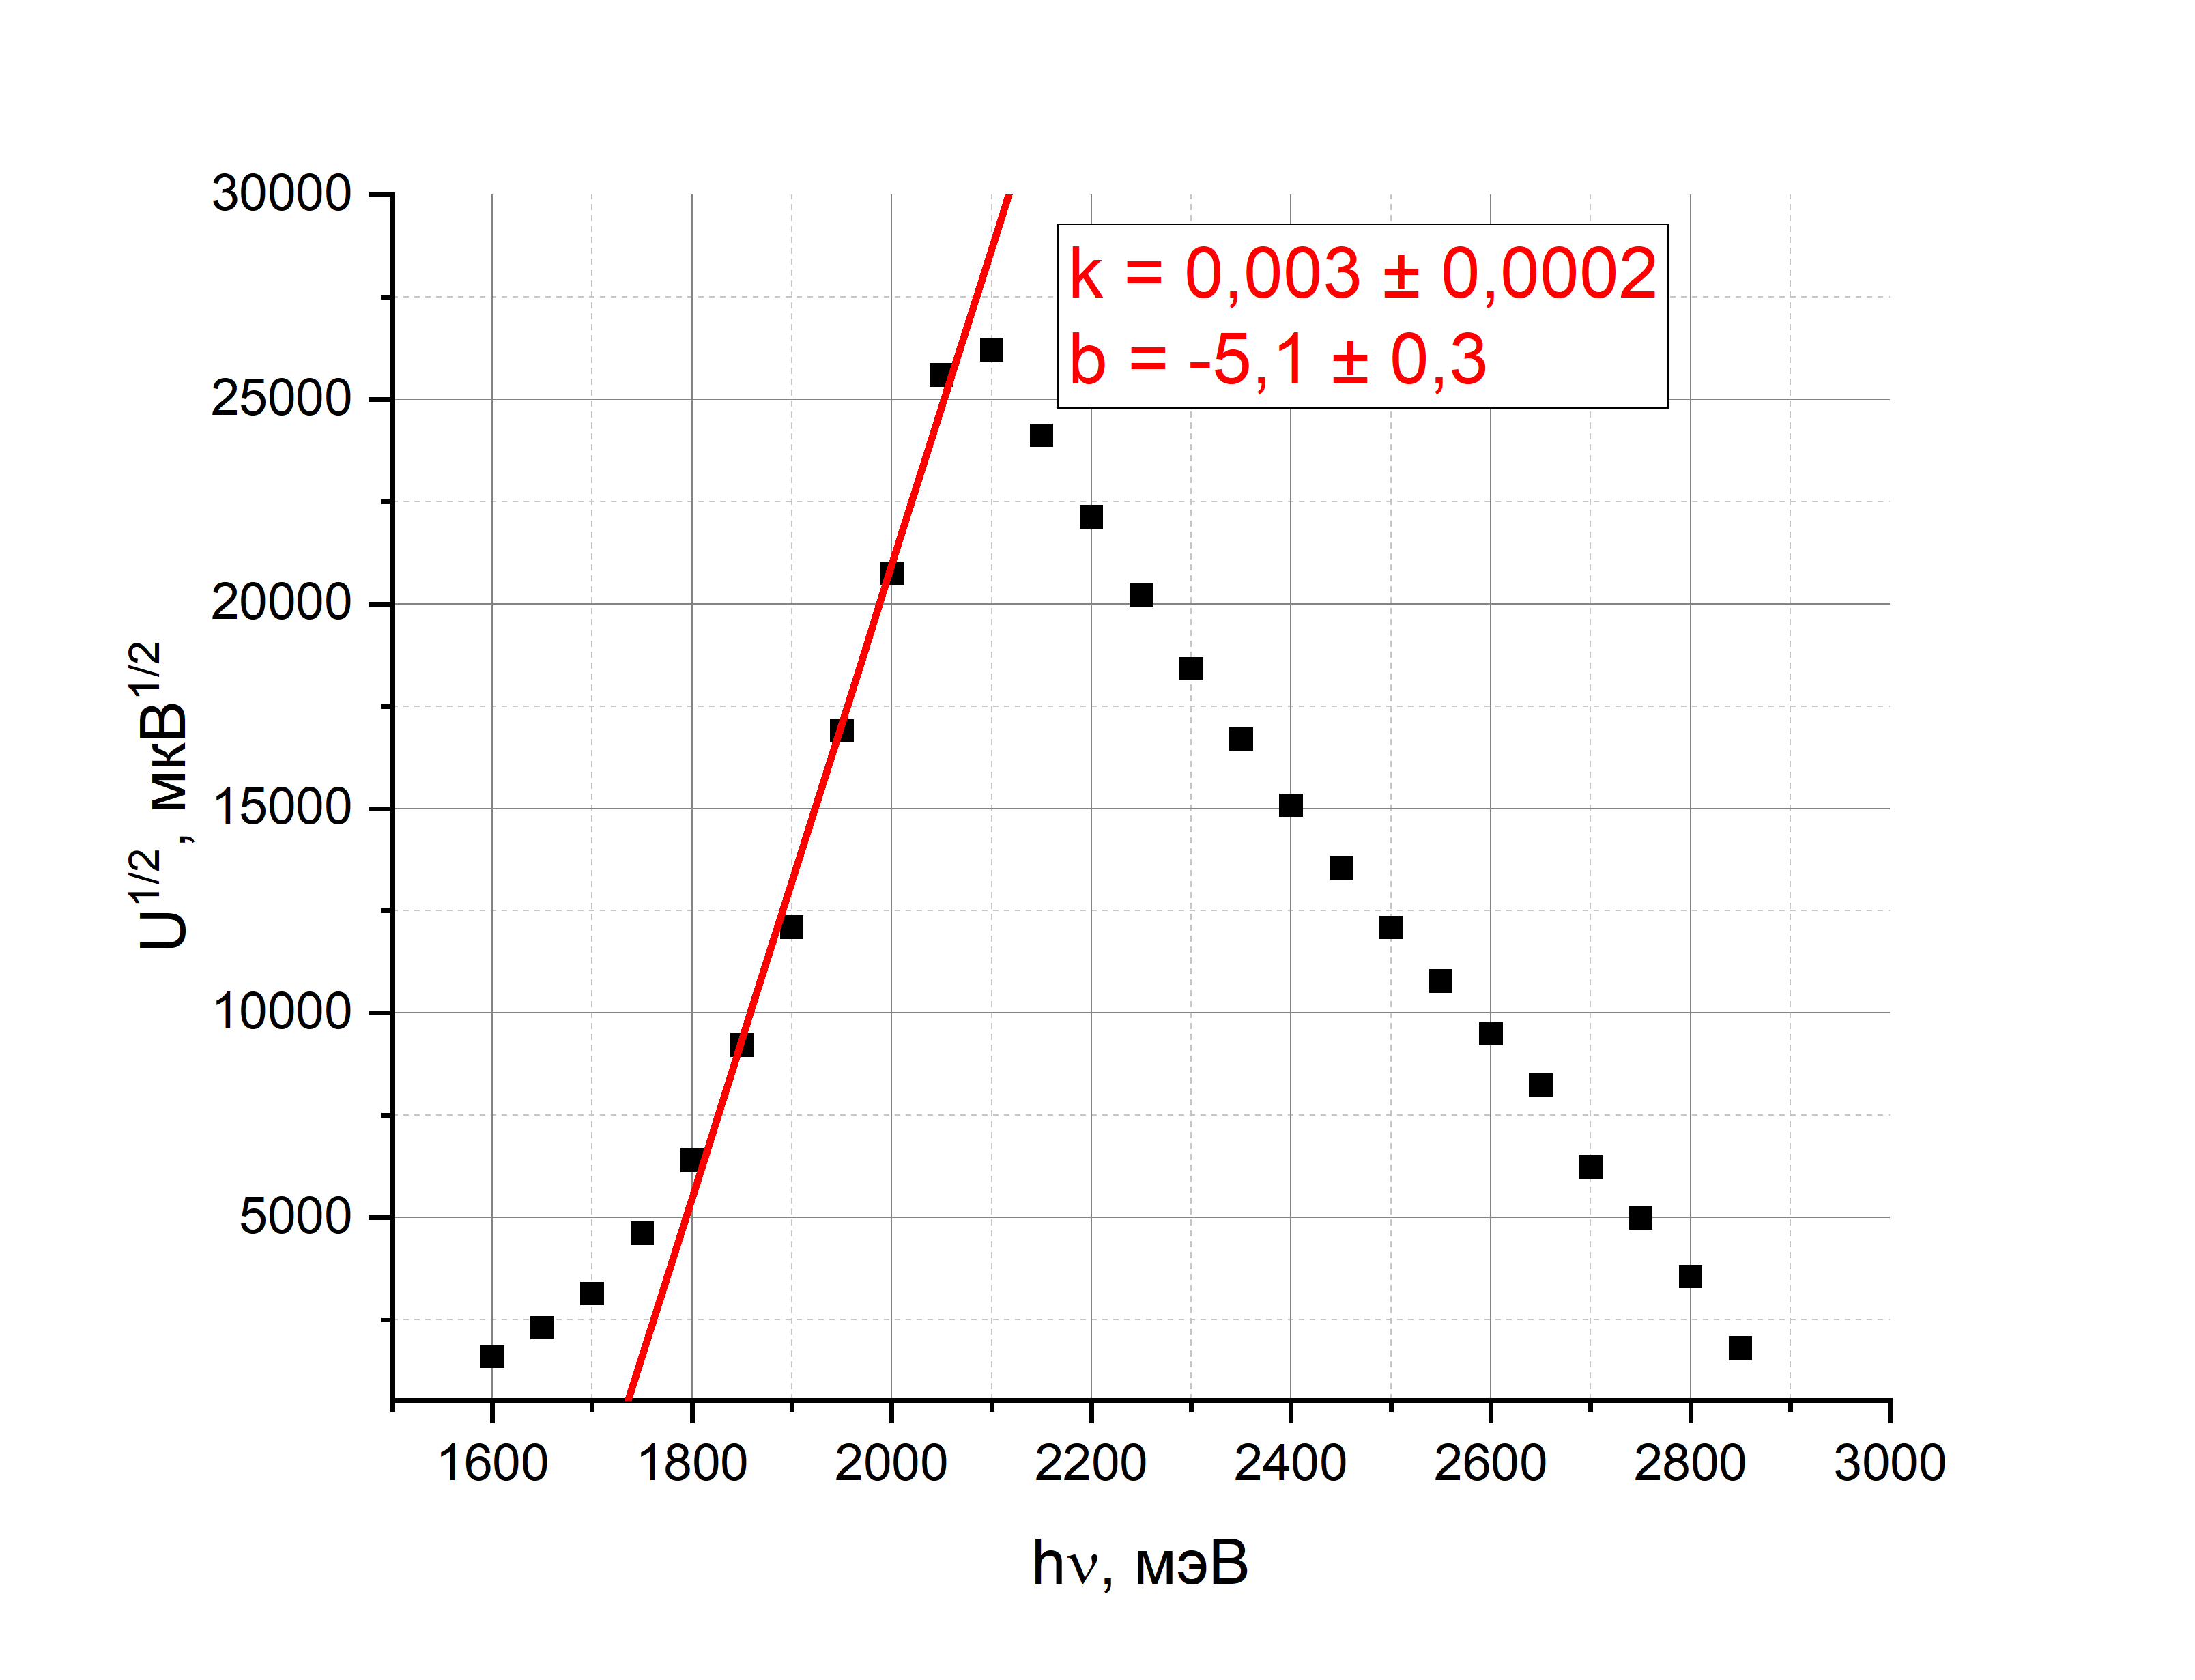
\includegraphics[width = 0.69 \textwidth]{CdSe.png}
    \caption{Определение ширины запрещенной зоны CdSe}
    \label{fig:CdSe}
\end{figure}

\newpage

Из рисунка $\ref{fig:CdSe}$ получаем точку пересечения прямой с осью $x$: $E_{g}^{CdSe} = (1730 \pm 60) \text{ мэВ}.$




\section{Вывод}

В ходе работы была определена ширина запрещенной зоны для двух образцов: $E_{g}^{Si} = (1100 \pm 50) \text{ мэВ}, E_{g}^{CdSe} = (1730 \pm 60) \text{ мэВ}.$ Табличные значения для этих величин: $E_{\text{табл}}^{Si} \sim 1.1 \text{ мэВ}, E_{\text{табл}}^{CdSe} \sim 1.7 \text{ мэВ}.$ Видим, что эксперимтально полученные значения соответствуют табличным.
\end{document}
